\documentclass[11pt]{book} % or report
\usepackage{amsmath}
\usepackage{amsfonts}
\usepackage{amssymb}
\usepackage{geometry}
\geometry{a4paper, margin=1in}
\usepackage{graphicx}
\usepackage[hidelinks]{hyperref}
\usepackage{amsthm}
\usepackage{tikz}
\usepackage{subcaption}
\usetikzlibrary{positioning}
\usepackage{pgfplots} 
\usepackage[ruled,vlined]{algorithm2e} 
\usepackage{dsfont}
\usepackage{graphicx}
\usepackage{mathdesign}
\usepackage{float}
\usepackage{todonotes} 
\usepackage{empheq}
\usepackage{array}
\usepackage[ruled,vlined]{algorithm2e} 
\usepackage[many]{tcolorbox}    	



\setlength{\parindent}{0pt}

% \let\stdsection\section
% \renewcommand\section{\newpage\stdsection}

\newcommand\mycommfont[1]{\footnotesize\ttfamily\textcolor{blue}{#1}}
\newcommand\defeq{\stackrel{\mathclap{\normalfont\mbox{def}}}{=}}
\SetCommentSty{mycommfont}

\DeclareMathOperator*{\argmax}{argmax}
\DeclareMathOperator*{\argmin}{argmin}

\newtheorem{theorem}{Theorem}[section]
\newtheorem{lemma}{Lemma}[section]
\newtheorem{definition}{Definition}[section]
\newtheorem{corollary}{Corollary}[section]
\newtheorem{claim}{claim}[section]
\newtheorem{example}{Example}[section]


\newtheorem*{claim*}{Claim}
\newtheorem*{lemma*}{Lemma}
\newtheorem*{corollary*}{Corollary}
\newtheorem*{remark*}{Remark}
\newtheorem*{example*}{Example}
\newtheorem*{examples*}{Examples}
\newtheorem*{definition*}{Definition}



\setcounter{tocdepth}{3}


\newtcolorbox{boxA}{
    fontupper = \bf,
    boxrule = 1.5pt,
    colframe = black 
}


\begin{document}

\begin{titlepage}
    \begin{center}
     {\huge\bfseries 
    Bound, Equalities and Inequalities     \\}
     % ----------------------------------------------------------------
     \vspace{1.5cm}
     {\Large\bfseries Hadar Tal}\\[5pt]
     hadar.tal@mail.huji.ac.il\\[14pt]
      % ----------------------------------------------------------------
     \vspace{2cm}
     {This paper is a summary of the educational materials and lectures from 
     \begin{itemize}
        \item \textbf{Wikipedia}
        \item \textbf{3Blue1Brown} YouTube channel
     \end{itemize}
     }

     \vfill
    {Winter 2024}
    \end{center}
\end{titlepage}


\frontmatter
\tableofcontents


\mainmatter

% * * * * * * * * * * * * * * * * * * * * * * * * 
% * * * * * * * * * * * * * * * * * * * * * * * * 
% * * * * * * * * * * * * * * * * * * * * * * * * 
% * * * * * * * * * * * * * * * * * * * * * * * * 
% * * * * * * * * * * * * * * * * * * * * * * * * 
% * * * * * * * * * * * * * * * * * * * * * * * * 
% * * * * * * * * * * * * * * * * * * * * * * * * 
% * * * * * * * * * * * * * * * * * * * * * * * * 
% * * * * * * * * * * * * * * * * * * * * * * * * 
% * * * * * * * * * * * * * * * * * * * * * * * * 
% * * * * * * * * * * * * * * * * * * * * * * * * 
% * * * * * * * * * * * * * * * * * * * * * * * * 
% * * * * * * * * * * * * * * * * * * * * * * * * 
% * * * * * * * * * * * * * * * * * * * * * * * * 
% * * * * * * * * * * * * * * * * * * * * * * * * 
% * * * * * * * * * * * * * * * * * * * * * * * * 
% * * * * * * * * * * * * * * * * * * * * * * * * 
% * * * * * * * * * * * * * * * * * * * * * * * * 
% * * * * * * * * * * * * * * * * * * * * * * * * 
\chapter{Bounds}


% * * * * * * * * * * * * * * * * * * * * * * * * 
% * * * * * * * * * * * * * * * * * * * * * * * * 
% * * * * * * * * * * * * * * * * * * * * * * * * 
% * * * * * * * * * * * * * * * * * * * * * * * * 
% * * * * * * * * * * * * * * * * * * * * * * * * 
% * * * * * * * * * * * * * * * * * * * * * * * * 
% * * * * * * * * * * * * * * * * * * * * * * * * 
% * * * * * * * * * * * * * * * * * * * * * * * * 
% * * * * * * * * * * * * * * * * * * * * * * * * 
% * * * * * * * * * * * * * * * * * * * * * * * * 
% * * * * * * * * * * * * * * * * * * * * * * * * 
% * * * * * * * * * * * * * * * * * * * * * * * * 
% * * * * * * * * * * * * * * * * * * * * * * * * 
% * * * * * * * * * * * * * * * * * * * * * * * * 
% * * * * * * * * * * * * * * * * * * * * * * * * 
% * * * * * * * * * * * * * * * * * * * * * * * * 
% * * * * * * * * * * * * * * * * * * * * * * * * 
% * * * * * * * * * * * * * * * * * * * * * * * * 
% * * * * * * * * * * * * * * * * * * * * * * * * 
\chapter{Equalities}

\section{Properties of Binomial Coefficients}

\subsection{Symmetry Rule for Binomial Coefficients}

\begin{boxA}
    \begin{theorem}
        For all $n, k \in \mathbb{N}$, the following holds
        \begin{equation}
            \binom{n}{k} = \binom{n}{n-k}
        \end{equation}
    \end{theorem}
\end{boxA}

\begin{proof}
    The proof is by definition of the binomial coefficient
    \begin{equation}
        \binom{n}{k} = \frac{n!}{k!(n-k)!}
    \end{equation}
    and the symmetry of the factorial function
    \begin{equation}
        n! = n \cdot (n-1) \cdot \ldots \cdot 2 \cdot 1 = 1 \cdot 2 \cdot \ldots \cdot (n-1) \cdot n = n!
    \end{equation}
    which implies that
    \begin{equation}
        \binom{n}{k} = \frac{n!}{k!(n-k)!} = \frac{n!}{(n-k)!k!} = \binom{n}{n-k}
    \end{equation}
\end{proof}

\begin{example*}
    The symmetry rule for binomial coefficients states that the number of ways to choose $k$ elements out of $n$ is the same as the number of ways to choose $n-k$ elements out of $n$.
\end{example*}


\subsection{Pascal's Rule for Binomial Coefficients}

\begin{boxA}
    \begin{theorem}
        For all $n, k \in \mathbb{N}$, the following holds
        \begin{equation}
            \binom{n}{k} = \binom{n-1}{k} + \binom{n-1}{k-1}
        \end{equation}
    \end{theorem}
\end{boxA}

\begin{proof}
    \begin{equation}
        \binom{n}{k} = \frac{n!}{k!(n-k)!} = \frac{(n-1)!}{k!(n-1-k)!} + \frac{(n-1)!}{(k-1)!(n-1-(k-1))!} = \binom{n-1}{k} + \binom{n-1}{k-1}
    \end{equation}
\end{proof}

\begin{example*}
    choosing a team of k players from n candidates: you can either include a specific player in your team and choose the rest 
    k-1 players from the remaining n-1 candidates, or not include that specific player, thus choosing all k players from the remaining n-1 candidates.
\end{example*}

\begin{figure}[H]
    \centering
    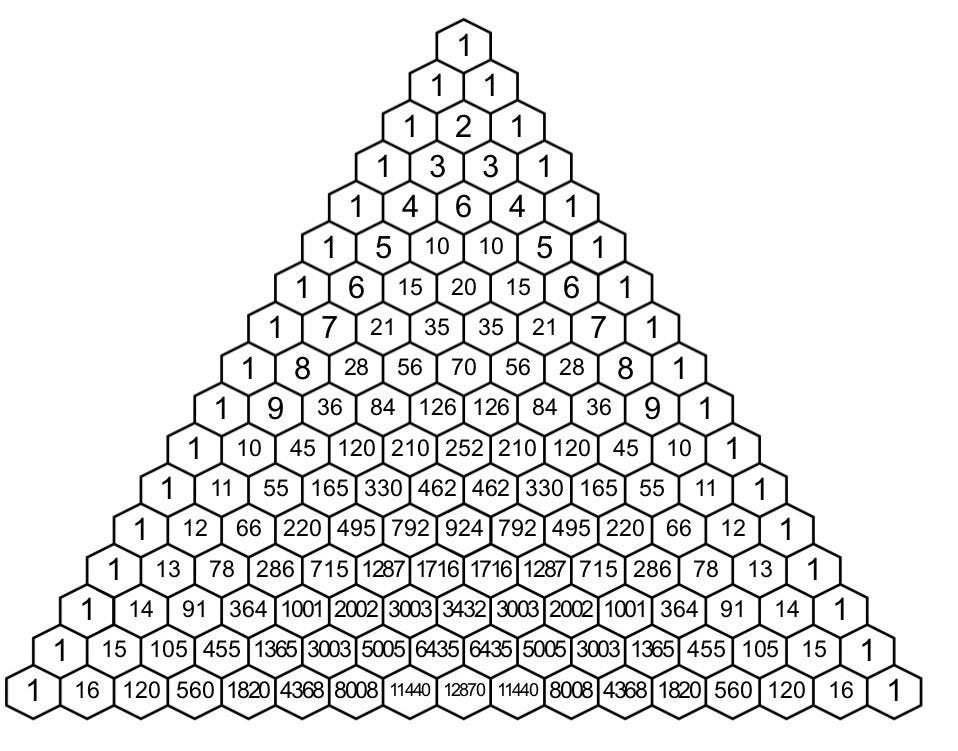
\includegraphics[width=0.4\textwidth]{figs/pascals_triangle.jpeg}
    \caption{Pascal's Triangle}
\end{figure}

\subsection{Sum of Binomial Coefficients over Lower Index}

\begin{boxA}
    \begin{theorem}
        For all $n\in \mathbb{N}$, the following holds
        \begin{equation}
            \sum_{i=0}^{n} \binom{n}{i} = 2^n
        \end{equation}
    \end{theorem}
\end{boxA}

\begin{proof}
    The proof is by induction on $n$. For $n=0$, the base case is
    \begin{equation}
        \sum_{i=0}^{0} \binom{0}{i} = \binom{0}{0} = 1 = 2^0
    \end{equation}
    For the induction step, assume that the theorem holds for $n=k$. Then
    \begin{equation}
        \sum_{i=0}^{k+1} \binom{k+1}{i} = \sum_{i=0}^{k+1} \left( \binom{k}{i} + \binom{k}{i-1} \right) = \sum_{i=0}^{k} \binom{k}{i} + \sum_{i=0}^{k} \binom{k}{i-1} = 2^k + 2^k = 2^{k+1}
    \end{equation}
\end{proof}

\begin{example*}
    The sum of binomial coefficients over the lower index is the same as counting all the subsets of a set of size $n$ which is $2^n$.
\end{example*}


\subsection{Factors of Binomial Coefficient}

\begin{boxA}
    \begin{theorem}
        For all $r \in \mathbb{R}, k \in \mathbb{Z}$, the following holds:
        \begin{equation}
            k \binom{r}{k} = r \binom{r-1}{k-1}
        \end{equation}
    \end{theorem}
\end{boxA}

\begin{proof}
    By definition, the binomial coefficient $\binom{r}{k}$ is given by
    \begin{equation}
        \binom{r}{k} = \frac{r!}{k!(r-k)!}.
    \end{equation}
    Multiplying both sides by $k$, we have
    \begin{equation}
        k \binom{r}{k} = k \frac{r!}{k!(r-k)!} = \frac{r!}{(k-1)!(r-k)!} = r \frac{(r-1)!}{(k-1)!(r-k)!} = r \binom{r-1}{k-1}.
    \end{equation}
\end{proof}

\begin{example*}
    Forming a committee of $k$ members from a group of $r$ individuals, with one member to be chosen as chairperson.
\end{example*}

\subsection{Increasing Sum of Binomial Coefficients}

\begin{boxA}
    \begin{theorem}
        For all $n\in \mathbb{N}$, the following holds
        \begin{equation}
            \sum_{k=0}^{n} k \binom{n}{k} = n 2^{n-1}
        \end{equation}
    \end{theorem}
\end{boxA}

\begin{proof}
    \begin{equation}
        \sum_{k=0}^{n} k \binom{n}{k} = \sum_{k=1}^{n} k \binom{n}{k} = \sum_{k=1}^{n} n \binom{n-1}{k-1} = n \sum_{k=1}^{n} \binom{n-1}{k-1} = n \sum_{k=0}^{n-1} \binom{n-1}{k} = n \cdot 2^{n-1}
    \end{equation}
\end{proof}

% * * * * * * * * * * * * * * * * * * * * * * * * 
% * * * * * * * * * * * * * * * * * * * * * * * * 
% * * * * * * * * * * * * * * * * * * * * * * * * 
% * * * * * * * * * * * * * * * * * * * * * * * * 
% * * * * * * * * * * * * * * * * * * * * * * * * 
% * * * * * * * * * * * * * * * * * * * * * * * * 
% * * * * * * * * * * * * * * * * * * * * * * * * 
% * * * * * * * * * * * * * * * * * * * * * * * * 
% * * * * * * * * * * * * * * * * * * * * * * * * 
% * * * * * * * * * * * * * * * * * * * * * * * * 
% * * * * * * * * * * * * * * * * * * * * * * * * 
% * * * * * * * * * * * * * * * * * * * * * * * * 
% * * * * * * * * * * * * * * * * * * * * * * * * 
% * * * * * * * * * * * * * * * * * * * * * * * * 
% * * * * * * * * * * * * * * * * * * * * * * * * 
% * * * * * * * * * * * * * * * * * * * * * * * * 
% * * * * * * * * * * * * * * * * * * * * * * * * 
% * * * * * * * * * * * * * * * * * * * * * * * * 
% * * * * * * * * * * * * * * * * * * * * * * * * 
\chapter{Inequalities}

\section{Vector Norms}

\begin{theorem}{\textbf{Cauchy-Schwarz Inequality}} \\
    Let $u, v$ be vectors of an inner product space. Then
    \begin{equation*}
        \left| \langle u, v \rangle \right|^2 \leq \left\| u \right\| \left\| v \right\|
    \end{equation*}
\end{theorem} 

\begin{theorem}{\textbf{Triangle Inequality}} \\
    Let $u, v$ be vectors of an inner product space. Then
    \begin{equation*}
        \left\| u + v \right\| \leq \left\| u \right\| + \left\| v \right\|
    \end{equation*}
\end{theorem}


\section{Probability}

\subsection{Markov's Inequality}

\begin{boxA}
    \begin{theorem}{\textbf{Markov's Inequality}} \\
        Let $X$ be a non-negative random variable and $a > 0$. Then
        \begin{equation*}
            P(X \geq a) \leq \frac{E[X]}{a}
        \end{equation*}
    \end{theorem}
\end{boxA}

\begin{proof}
    \begin{equation}
        E[X] = \int_{0}^{\infty} x f(x) dx \geq \int_{a}^{\infty} x f(x) dx \geq \int_{a}^{\infty} a f(x) dx = a \int_{a}^{\infty} f(x) dx = a P(X \geq a)
    \end{equation}
\end{proof}

\subsection{Chebyshev's Inequality}

\begin{boxA}
    \begin{theorem}{\textbf{Chebyshev's Inequality}} \\
        Let $X$ be a random variable with mean $\mu$ and variance $\sigma^2$. Then
        \begin{equation*}
            P(|X - \mu| \geq a) \leq \frac{\sigma^2}{a^2}
        \end{equation*}
    \end{theorem}
\end{boxA}

\begin{proof}
    \begin{equation}
        P(|X - \mu| \geq a) = P((X - \mu)^2 \geq a^2) \leq \frac{E[(X - \mu)^2]}{a^2} = \frac{\sigma^2}{a^2}
    \end{equation}
\end{proof}


\subsection{Chernoff Bound for Sum of Independent Bernoulli Variables}

\begin{boxA}
    \begin{theorem}{\textbf{Chernoff Bound}}
        Let \(X_1, X_2, \ldots, X_n\) be independent Bernoulli random variables with \(X_i \sim \text{Bernoulli}(p_i)\) and \( \Pr(X_i = 1) = p_i \). Define \( \mu = E\left[\sum_{i=1}^n X_i\right] = \sum_{i=1}^n p_i \). Then for any \( \delta > 0 \), the following bounds hold:
        \begin{equation*}
            \Pr\left(\sum_{i=1}^n X_i \geq (1 + \delta) \mu\right) \leq \left(\frac{e^\delta}{(1+\delta)^{1+\delta}}\right)^\mu, \quad \text{if } \delta > 0
        \end{equation*}
        \begin{equation*}
            \Pr\left(\sum_{i=1}^n X_i \leq (1 - \delta) \mu\right) \leq \left(\frac{e^{-\delta}}{(1-\delta)^{1-\delta}}\right)^\mu, \quad \text{if } 0 < \delta < 1
        \end{equation*}
    \end{theorem}
\end{boxA}

\begin{proof}
    Define \( t = \log(1 + \delta) \) for the upper tail bound and \( t = -\log(1 - \delta) \) for the lower tail bound. By using the moment-generating function approach, we have:
    \begin{equation}
        E[e^{tX_i}] = p_i e^t + (1 - p_i) = 1 + p_i(e^t - 1) \leq e^{p_i(e^t - 1)}
    \end{equation}
    Thus, for the upper bound:
    \begin{equation}
        \begin{aligned}
            E\left[e^{t\sum_{i=1}^n X_i}\right] = \prod_{i=1}^n E[e^{tX_i}] = \prod_{i=1}^n \left(1 + p_i(e^t - 1)\right) \\
            \leq \prod_{i=1}^n e^{p_i(e^t - 1)} = e^{\sum_{i=1}^n p_i(e^t - 1)} = e^{\mu (e^t - 1)} 
        \end{aligned}
    \end{equation}
    \begin{equation}
        \Pr\left(\sum_{i=1}^n X_i \geq (1+\delta)\mu\right) \leq \frac{e^{\mu(e^t - 1)}}{e^{t(1+\delta)\mu}} = e^{-\mu t \delta} \left(\frac{e^t}{1+\delta}\right)^\mu
    \end{equation}
    Simplifying further using Taylor series approximations and properties of logarithms, we obtain the upper bound as stated in the theorem.

    The proof for the lower bound follows similarly, using \( t = -\log(1 - \delta) \) and applying analogous steps.
\end{proof}

\textbf{Remarks:}
This proof illustrates the power of the Chernoff bound for providing exponentially decreasing bounds on the tail probabilities of the sum of independent Bernoulli trials, particularly useful in scenarios involving large numbers of independent events or trials.


\begin{boxA}
    \begin{theorem}
        Let \(X_1, X_2, \ldots, X_n\) be independent Bernoulli random variables where each \(X_i\) takes values in \(\{0, 1\}\). Define \(Z_n = \sum_{i=1}^n X_i\) and \(\mu = E[Z_n]\). Then for any \(\delta > 0\), it holds that:
        \begin{equation}
            \Pr(|Z_n - \mu| \geq \delta \mu) \leq 2 e^{-\frac{\delta^2 \mu}{2}}.
        \end{equation}
    \end{theorem}    
\end{boxA}







\end{document}